\documentclass[11pt, addpoints, answers]{exam}

\usepackage{amsmath, amssymb, euler}
\usepackage{xcolor}
\usepackage{algorithm, algorithmicx, algpseudocode}
\usepackage{tikz, tikz-qtree, drawstack}
\usepackage[shortlabels]{enumitem}

\usetikzlibrary{graphs}
\tikzset{every tree node/.style={minimum width=2em,draw,circle},
	blank/.style={draw=none},
	edge from parent/.style=
	{draw,edge from parent path={(\tikzparentnode) -- (\tikzchildnode)}},
	level distance=1.2cm}

% For inserting code snippets.
\usepackage{listings}
\lstset{
    columns = fixed,
    basewidth = {0.5em},
    breaklines = true,
    backgroundcolor = \color{white},
    keywordstyle = \color[RGB]{40, 40, 255},
    numberstyle = \footnotesize\color{darkgray},
    commentstyle = \ttfamily\color{violet},
    basicstyle = \ttfamily,
    stringstyle = \ttfamily\color[RGB]{128, 0, 0},
    showstringspaces = false,
    language = {[11]C++},
    escapechar = \@
}
\lstnewenvironment{cpp}[1][]{\lstset{language = {[11]C++}, #1}}{}

\usepackage{tikz}

% headers, footers, titles
\newcommand{\CourseName}{CS101 Algorithms and Data Structures}
\newcommand{\HomeworkNO}{Homework 4}
\newcommand{\DueDate}{Due date: 23:59, October 16th, 2022}

\pagestyle{headandfoot}
\runningheadrule
\runningheader{\CourseName}{\HomeworkNO}{\DueDate}
\runningfooter{}{\thepage}{}

\title{
	\CourseName\\
	Fall 2022\\
	\HomeworkNO
}
\author{}
\date{\DueDate}

% formats of questions, choices, points, etc.
\qformat{\bf\thequestion. (\totalpoints\ points) \thequestiontitle\hfill}
\pointname{'}
\CorrectChoiceEmphasis{\bf\color{blue}}

% We frequently use this font.
\newcommand{\ttt}{\texttt}
\newcommand{\blue}[1]{\textcolor{blue}{#1}}
\newcommand{\bluett}[1]{\blue{\ttt{#1}}}

\begin{document}

\maketitle

\begin{enumerate}
	\item Please write your solutions in English.
	\item Submit your solutions to gradescope.com.
	\item Set your FULL name to your Chinese name and your STUDENT ID correctly in Account Settings.
	\item If you want to submit a handwritten version, scan it clearly. \ttt{CamScanner} is recommended.
	\item When submitting, match your solutions to the problems correctly.
	\item No late submission will be accepted.
	\item Violations to any of the above may result in zero points.
\end{enumerate}

\newpage


{\large\textbf{Notes}:}

\begin{enumerate}
	\item Some problems in this homework requires you to design Divide and Conquer algorithm. When grading these problems, we will put more emphasis on how you reduce a problem to a smaller size problem and how to combine their solutions with Divide and Conquer strategy. 
	\item Your answer for these problems {\color{red}\textbf{should}} include:
	\begin{enumerate}
		\item {\color{red}Algorithm Design}
		\item {\color{red}Time Complexity Analysis}
		\item Pseudocode (Optional)
	\end{enumerate}
    \item Your answer for these problems is {\color{red}not allowed to include real C or C++ code}.
	\item In Algorithm Design, you should describe each step of your algorithm clearly.
	\item Unless required, writing pseudocode is optional. If you write pseudocode, please give some additional descriptions if the pseudocode is not obvious.
	\item You are recommended to finish the algorithm design part of this homework with \LaTeX.
\end{enumerate}

\newpage

\begin{questions}

\titledquestion{Maximum Subarray Problem}

Given an array $A=\langle A_1, \dots, A_n\rangle$ of $n$ elements, please design a dynamic programming algorithm to find a contiguous subarray whose sum is maximum.

\vspace{0.05in}
{\large\textbf{Notes:}} \textcolor{red}{(MUST READ!)}

\begin{enumerate}
	\item Problems in this homework require you to design \textbf{dynamic programming} algorithms. When grading these problems, we will put more emphasis on how you define your subproblems, whether your Bellman equation is correct and correctness of your complexity analysis.
	\item \textbf{Define your subproblems clearly.} Your definition should include the variables you choose for each subproblem and a brief description of your subproblem in terms of the chosen variables.
	\item Your \textbf{Bellman equation} should be a recurrence relation whose \textbf{base case} is well-defined. You can briefly \textbf{explain each term in the equation} if necessary, which might improve the readability of your solution and help TAs grade it. 
	\item Analyze the \textbf{runtime complexity} of your algorithm in terms of $\Theta(\cdot)$ notation.
	\item You only need to calculate the optimal value in each problem of this homework, and you don't have to back-track to find the optimal solution.
\end{enumerate}

% utilities you might need for wrting Bellman equations
\newcommand{\maxi}[2]{\max\left\{#1,\ #2\right\}}	% usage: \maxi{a}{b}
\newcommand{\maxt}[3]{\max\begin{cases}#1\\#2\\#3\end{cases}}	% usage: \maxt{a}{b}{c}
\newcommand{\mini}[2]{\min\left\{#1,\ #2\right\}}	% usage: \mini{a}{b}
\newcommand{\mint}[3]{\min\begin{cases}#1\\#2\\#3\end{cases}}	% usage: \mint{a}{b}{c}
\newcommand{\case}[1]{\text{if}\ #1}	% usage: \case{$i > 1$}
\newcommand{\otherwise}{\text{otherwise}}	% usage: \otherwise

\vspace{0.05in}
\begin{parts}
	\part[0] Define your subproblem for this question.
	\begin{solution}
		$OPT(i)=$ the maximum sum of subarrays of $A$ ending with $A_i$.
	\end{solution}

	\part[0] Give your Bellman equation to solve the subproblems.
	\begin{solution}
		\[
			OPT(i)=
			\begin{cases}
				A_1                      & \case{i=1} \\
				\maxi{A_i}{A_i+OPT(i-1)} & \case{i>1}
			\end{cases}
		\]
		\paragraph{Explanation:} (NOT Required)
		\begin{itemize}
			\item The $1$st term in $\max$: only take $A_i$
			\item The $2$nd term in $\max$: take $A_i$ together with the best subarray ending with $A_{i-1}$
		\end{itemize}
	\end{solution}

	\part[0] What is the answer to this question in terms of the subproblems?
	\begin{solution}
		\[ \max_{i\in\{1, 2, \dots, n\}} OPT(i) \]
	\end{solution}

	\part[0] What is the runtime complexity of your algorithm?
	\begin{solution}
		$\Theta(n)$
	\end{solution}
\end{parts}

\newpage

\titledquestion{Trees}

Each question has \textbf{one or more than one} correct answer(s). Please answer the following questions \textbf{according to  the definition specified in the lecture slides}.

%%%%%%%%%%%%%%%%%%%%%%%%%%%%%%%%%%%%%%%%%%%%%%%%%%%%%%%%%%%%%%%%%%%%%%%%%%%
% Note: The `LaTeX' way to answer a multiple-choices question is to replace `\choice'
% with `\CorrectChoice', as what you did in the previous questions. However, there are 
% still many students who would like to handwrite their homework. To make TA's work 
% easier, you have to fill your selected choices in the table below, no matter whether 
% you use LaTeX or not.
%%%%%%%%%%%%%%%%%%%%%%%%%%%%%%%%%%%%%%%%%%%%%%%%%%%%%%%%%%%%%%%%%%%%%%%%%%%

\begin{table}[htbp]
	\centering
	\begin{tabular}{|p{2cm}|p{2cm}|p{2cm}|}
		\hline
		(a) & (b) & (c) \\
		\hline
		%%%%%%%%%%%%%%%%%%%%%%%%%%%%%%%%%%%%%%%%%%%%%%%%%%%%%%%%%%
		% YOUR ANSWER HERE.
		 ABD   &  A   &  A   \\
		%%%%%%%%%%%%%%%%%%%%%%%%%%%%%%%%%%%%%%%%%%%%%%%%%%%%%%%%%%
		\hline
	\end{tabular}
\end{table}

\begin{parts}
	\part[3] Which of the following statements is(are) \textbf{false}?

	\begin{choices}
        \CorrectChoice Nodes with the same depth are siblings.
        \CorrectChoice Each node in a tree has exactly one parent pointing to it.
        \choice Given any node $a$ within a tree, the collection of $a$ and all of its descendants is a subtree of the tree with root $a$.
        \CorrectChoice The root node cannot be the descendant of any node.
        \choice Nodes with degree zero are called leaf nodes.
        \choice Any tree can be converted into a forest by removing the root node.
	\end{choices}

	\part[3] {Given the following pseudo-code, what kind of traversal does it implement?}

    \begin{center}
    \begin{minipage}{.7\linewidth}
        \begin{algorithm}[H]
            \begin{algorithmic}[1]
                \Function {order}{node}			
                \State visit(node)
        
                \If{node has left child}
                \State order(node.left)
                \EndIf
        
                \If{node has right child}
                \State order(node.right)
                \EndIf 
        
                \EndFunction
            \end{algorithmic}
        \end{algorithm}
    \end{minipage}
    \end{center}

	\begin{choices}
        \CorrectChoice Preorder depth-first traversal
        \choice Postorder depth-first traversal
        \choice Inorder depth-first traversal
        \choice Breadth-first traversal
	\end{choices}

    \newpage

	\part[3] Which traversal strategy should we use if we want to print the hierarchical structure?

    \begin{figure}[h]
        \centering
        \includegraphics[width=0.27\linewidth]{hierarchy}
    \end{figure}
		
	\begin{choices}
        \CorrectChoice CorrectChoice depth-first traversal
        \choice Postorder depth-first traversal
        \choice Inorder depth-first traversal
        \choice Breadth-first traversal
	\end{choices}
\end{parts}

\newpage

\titledquestion{Tree Properties}

Answer the following questions for the tree shown below \textbf{according to  the definition specified in the lecture slides}. Please specify:

\begin{center}
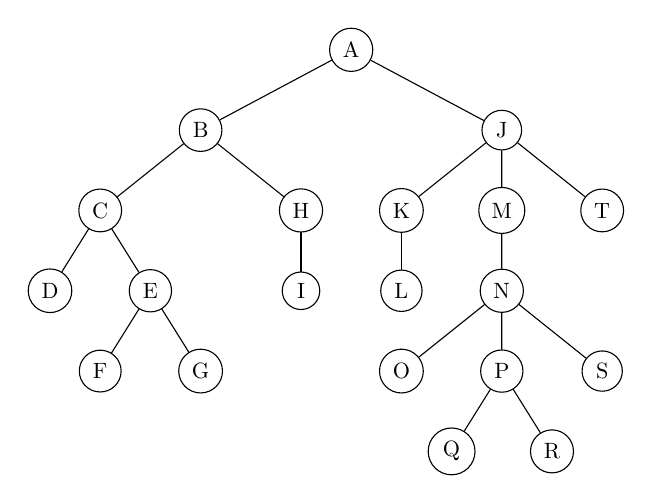
\begin{tikzpicture}[scale=0.85, every node/.style={scale=0.8}]
    \node [circle,draw] {A}
    child {node [circle,draw] {B}
        child {node [circle,draw] {C}
            child {node [circle,draw] {D}}
            child {node [circle,draw] {E}
                child {node [circle,draw] {F}}
                child {node [circle,draw] {G}}
            }
        }
        child [missing] {}
        child {node [circle,draw] {H}
            child {node [circle,draw] {I}}
        }
    }	
    child [missing] {}	
    child [missing] {}	
    child {node [circle,draw] {J}
        child {node [circle,draw] {K}
            child {node [circle,draw] {L}}
        }
        child {node [circle,draw] {M}
            child {node [circle,draw] {N}
                child {node [circle,draw] {O}}
                child {node [circle,draw] {P}
                    child {node [circle,draw] {Q}}
                    child {node [circle,draw] {R}}	
                }
                child {node [circle,draw] {S}}
            }
        }
        child {node [circle,draw] {T}}
    };
\end{tikzpicture}
\end{center}

\begin{parts}
    \part[2] The \textbf{children} of the \textbf{root node} with their \textbf{degree} respectively.
    \begin{solution}
        %%%%%%%%%%%%%%%%%%%%%%%%%%%%%%%%%%%%%%%%%%%%%%%%%
        % Replace `\vspace{2in}' with your answer.
        %\vspace{1in}
        B, J

        deg(B)=2, deg(J)=3
        %%%%%%%%%%%%%%%%%%%%%%%%%%%%%%%%%%%%%%%%%%%%%%%%%
    \end{solution}
    \part[2] All \textbf{leaf nodes} in the forest with their \textbf{depth} if we remove A and the node with the lexicographically smallest character in a tree is taken as the root node.
    \begin{solution}
        %%%%%%%%%%%%%%%%%%%%%%%%%%%%%%%%%%%%%%%%%%%%%%%%%
        % Replace `\vspace{2in}' with your answer.
        %\vspace{1in}
        D, F, G, I, L, O, Q, R, S, T

        height(T) = 1

        height(D) = height(I) = height(L) = 2

        height(F) = height(G) = height(O) = height(S) = 3

        height(Q) = height(R) = 4
        %%%%%%%%%%%%%%%%%%%%%%%%%%%%%%%%%%%%%%%%%%%%%%%%%
    \end{solution}
    \part[2] The \textbf{height} of the tree.
    \begin{solution}
        %%%%%%%%%%%%%%%%%%%%%%%%%%%%%%%%%%%%%%%%%%%%%%%%%
        % Replace `\vspace{2in}' with your answer.
        %\vspace{1in}
        height = max\{depth(v) | v \(\in\) V\} = 5

        so height = 5
        %%%%%%%%%%%%%%%%%%%%%%%%%%%%%%%%%%%%%%%%%%%%%%%%%
    \end{solution}

    \newpage

    \part[2] The \textbf{ancestors} of R. 
    \begin{solution}
        %%%%%%%%%%%%%%%%%%%%%%%%%%%%%%%%%%%%%%%%%%%%%%%%%
        % Replace `\vspace{2in}' with your answer.
        %\vspace{1in}
        R, P, N, M, J, A
        %%%%%%%%%%%%%%%%%%%%%%%%%%%%%%%%%%%%%%%%%%%%%%%%%
    \end{solution}
    \part[2] The \textbf{descendants} of L.
    \begin{solution}
        %%%%%%%%%%%%%%%%%%%%%%%%%%%%%%%%%%%%%%%%%%%%%%%%%
        % Replace `\vspace{2in}' with your answer.
        %\vspace{1in}
        L
        %%%%%%%%%%%%%%%%%%%%%%%%%%%%%%%%%%%%%%%%%%%%%%%%%
    \end{solution}
    \part[2] The \textbf{path} from E to S.
    \begin{solution}
        %%%%%%%%%%%%%%%%%%%%%%%%%%%%%%%%%%%%%%%%%%%%%%%%%
        % Replace `\vspace{2in}' with your answer.
        %\vspace{1in}
        \(E \to C \to B \to A \to J \to M \to N \to S\)
        %%%%%%%%%%%%%%%%%%%%%%%%%%%%%%%%%%%%%%%%%%%%%%%%%
    \end{solution}
\end{parts}

\newpage

\titledquestion{Tree Structure and Traversal}

Answer the following questions for the tree shown below \textbf{according to  the definition specified in the lecture slides}.

Note: Form your answer in the following steps.
\begin{enumerate}[1.]
    \item Decide on an appropriate \textbf{data structure} to implement the traversal.
    \item When you are pushing the children of a node into a \textbf{queue}, please push them alphabetically; when you are pushing the children of a node into a \textbf{stack}, please push them in a reversely alphabetical order.
    \item \textbf{Show all current elements in your data structure at each step} clearly. \textbf{Popping a node} or \textbf{pushing a sequence of children} can be considered as one single step.
    \item \textbf{Write down your traversal sequence} i.e. the order that you pop elements out of the data structure.
\end{enumerate}

Please refer to the examples displayed in the lecture slide for detailed implementation of traversal in a tree using the data structure.

\begin{parts}
    \part[4] Use stack to run \textbf{Preorder Depth First Traversal} in the tree with root E and you should fill stack step by step and then write down the traversal sequence. 
    \begin{center}
        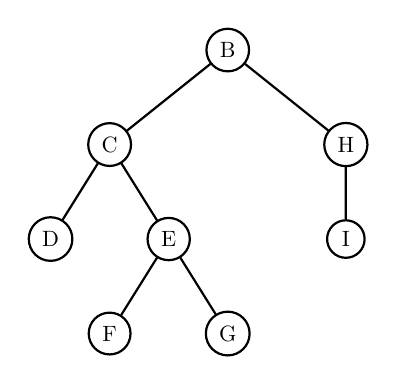
\begin{tikzpicture}[thick,scale=1.0, every node/.style={scale=0.8}]
            \node [circle,draw] {B}
            child {node [circle,draw] {C}
                    child {node [circle,draw] {D}}
                    child {node [circle,draw] {E}
                        child {node [circle,draw] {F}}
                        child {node [circle,draw] {G}}
                    }
            }	
            child [missing] {}
            child {node [circle,draw] {H}
                child {node [circle,draw] {I}}
            };
        \end{tikzpicture}
    \end{center}

    \begin{solution}

        \begin{minipage}{.14\linewidth}
            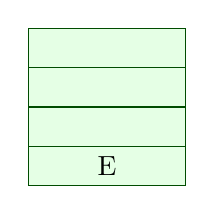
\begin{tikzpicture}[scale=0.5]
                \cell{}
                \cell{}
                \cell{}
                \cell{E}
            \end{tikzpicture}
        \end{minipage}
        $\to$
        \begin{minipage}{.14\linewidth}
            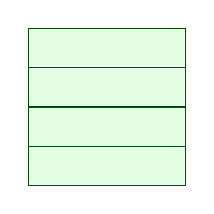
\begin{tikzpicture}[scale=0.5]
                \cell{}
                \cell{}
                \cell{}
                \cell{}
            \end{tikzpicture}
        \end{minipage}
        $\to$
        \begin{minipage}{.14\linewidth}
            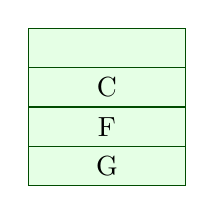
\begin{tikzpicture}[scale=0.5]
                \cell{}
                \cell{C}
                \cell{F}
                \cell{G}
            \end{tikzpicture}
        \end{minipage}
        $\to$
        \begin{minipage}{.14\linewidth}
            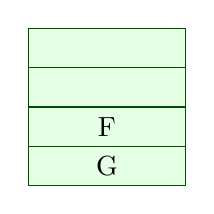
\begin{tikzpicture}[scale=0.5]
                \cell{}
                \cell{}
                \cell{F}
                \cell{G}
            \end{tikzpicture}
        \end{minipage}
        $\to$
        \begin{minipage}{.14\linewidth}
            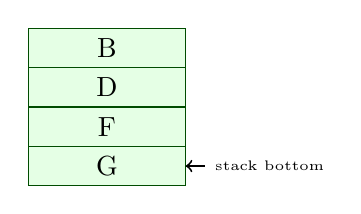
\begin{tikzpicture}[scale=0.5]
                \cell{B}
                \cell{D}
                \cell{F}
                \cell{G}\cellptr{\tiny {stack bottom}}
            \end{tikzpicture}
        \end{minipage}
        $\to$

        \begin{minipage}{.14\linewidth}
            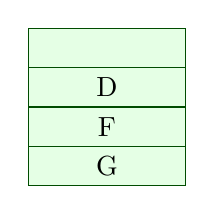
\begin{tikzpicture}[scale=0.5]
                \cell{}
                \cell{D}
                \cell{F}
                \cell{G}
            \end{tikzpicture}
        \end{minipage}
        $\to$
        \begin{minipage}{.14\linewidth}
            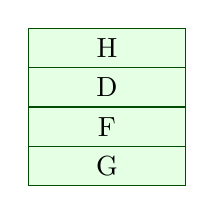
\begin{tikzpicture}[scale=0.5]
                \cell{H}
                \cell{D}
                \cell{F}
                \cell{G}
            \end{tikzpicture}
        \end{minipage}
        $\to$
        \begin{minipage}{.14\linewidth}
            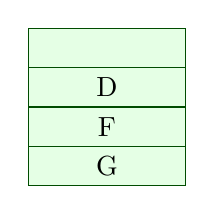
\begin{tikzpicture}[scale=0.5]
                \cell{}
                \cell{D}
                \cell{F}
                \cell{G}
            \end{tikzpicture}
        \end{minipage}
        $\to$
        \begin{minipage}{.14\linewidth}
            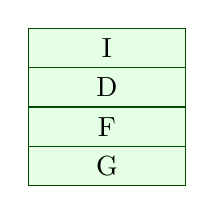
\begin{tikzpicture}[scale=0.5]
                \cell{I}
                \cell{D}
                \cell{F}
                \cell{G}
            \end{tikzpicture}
        \end{minipage}
        $\to$
        \begin{minipage}{.14\linewidth}
            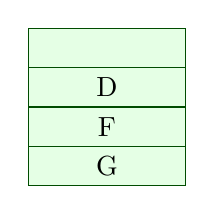
\begin{tikzpicture}[scale=0.5]
                \cell{}
                \cell{D}
                \cell{F}
                \cell{G} 
            \end{tikzpicture}
        \end{minipage}
        $\to$

        \begin{minipage}{.14\linewidth}
            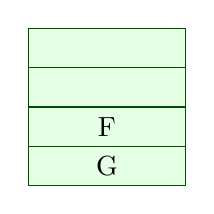
\begin{tikzpicture}[scale=0.5]
                \cell{}
                \cell{}
                \cell{F}
                \cell{G}
            \end{tikzpicture}
        \end{minipage}
        $\to$
        \begin{minipage}{.14\linewidth}
            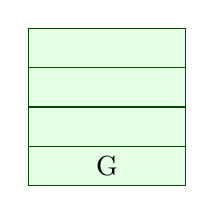
\begin{tikzpicture}[scale=0.5]
                \cell{}
                \cell{}
                \cell{}
                \cell{G}
            \end{tikzpicture}
        \end{minipage}
        $\to$
        \begin{minipage}{.14\linewidth}
            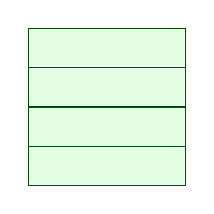
\begin{tikzpicture}[scale=0.5]
                \cell{}
                \cell{}
                \cell{}
                \cell{}
            \end{tikzpicture}
        \end{minipage}
        $\to$
        \begin{minipage}{.14\linewidth}
            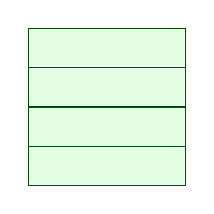
\begin{tikzpicture}[scale=0.5]
                \cell{}
                \cell{}
                \cell{}
                \cell{}
            \end{tikzpicture}
        \end{minipage}
        $\to$
        \begin{minipage}{.14\linewidth}
            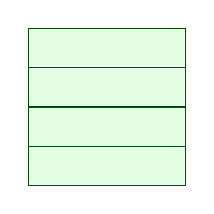
\begin{tikzpicture}[scale=0.5]
                \cell{}
                \cell{}
                \cell{}
                \cell{}
            \end{tikzpicture}
        \end{minipage}

        Traversal Sequence: E, C, B, H, I, D, F, G
    \end{solution}
    
    \newpage
    \part[4] Use queue to run \textbf{Breadth First Traversal} in the tree with root P and you should fill queue step by step and then write down the traversal sequence. 

    \begin{center}
        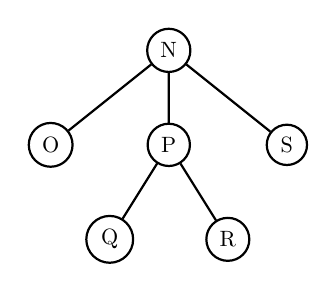
\begin{tikzpicture}
            [thick,scale=1, every node/.style={scale=0.8}]
            \node [circle,draw] {N}
                child {node [circle,draw] {O}}
                child {node [circle,draw] {P}
                    child {node [circle,draw] {Q}}
                    child {node [circle,draw] {R}}	
                }
                child {node [circle,draw] {S}};
        \end{tikzpicture}
    \end{center}
    \begin{solution}\par
        \begin{minipage}{.14\linewidth}
            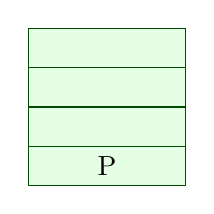
\begin{tikzpicture}[scale=0.5]
                \cell{}
                \cell{}
                \cell{}
                \cell{P}
            \end{tikzpicture}
        \end{minipage}
        $\to$
        \begin{minipage}{.14\linewidth}
            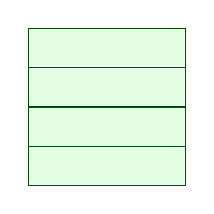
\begin{tikzpicture}[scale=0.5]
                \cell{}
                \cell{}
                \cell{}
                \cell{}
            \end{tikzpicture}
        \end{minipage}
        $\to$
        \begin{minipage}{.14\linewidth}
            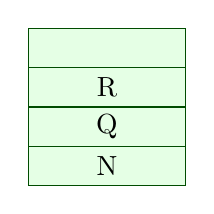
\begin{tikzpicture}[scale=0.5]
                \cell{}
                \cell{R}
                \cell{Q}
                \cell{N}
            \end{tikzpicture}
        \end{minipage}
        $\to$
        \begin{minipage}{.14\linewidth}
            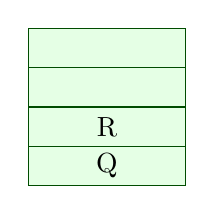
\begin{tikzpicture}[scale=0.5]
                \cell{}
                \cell{}
                \cell{R}
                \cell{Q}
            \end{tikzpicture}
        \end{minipage}
        $\to$
        \begin{minipage}{.14\linewidth}
            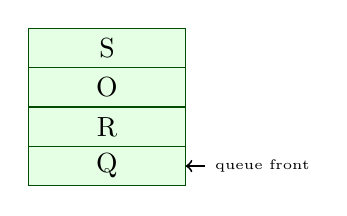
\begin{tikzpicture}[scale=0.5]
                \cell{S}
                \cell{O}
                \cell{R}
                \cell{Q}\cellptr{\tiny {queue front}}
            \end{tikzpicture}
        \end{minipage}
        $\to$

        \begin{minipage}{.14\linewidth}
            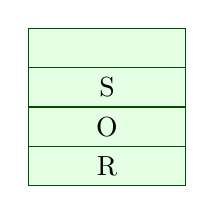
\begin{tikzpicture}[scale=0.5]
                \cell{}
                \cell{S}
                \cell{O}
                \cell{R}
            \end{tikzpicture}
        \end{minipage}
        $\to$
        \begin{minipage}{.14\linewidth}
            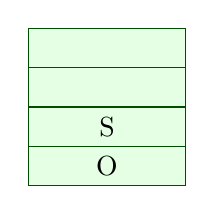
\begin{tikzpicture}[scale=0.5]
                \cell{}
                \cell{}
                \cell{S}
                \cell{O}
            \end{tikzpicture}
        \end{minipage}
        $\to$
        \begin{minipage}{.14\linewidth}
            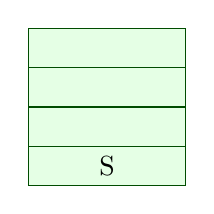
\begin{tikzpicture}[scale=0.5]
                \cell{}
                \cell{}
                \cell{}
                \cell{S}
            \end{tikzpicture}
        \end{minipage}
        $\to$
        \begin{minipage}{.14\linewidth}
            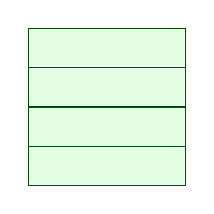
\begin{tikzpicture}[scale=0.5]
                \cell{}
                \cell{}
                \cell{}
                \cell{}
            \end{tikzpicture}
        \end{minipage}
        $\to$
        \begin{minipage}{.14\linewidth}
            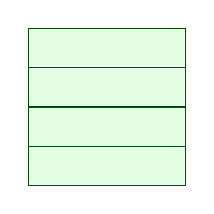
\begin{tikzpicture}[scale=0.5]
                \cell{}
                \cell{}
                \cell{}
                \cell{} 
            \end{tikzpicture}
        \end{minipage}

        Traversal Sequence: P, N, Q, R, O, S
    \end{solution}

\end{parts}

\newpage

\titledquestion{Recurrence Relations}

For each question, find the asymptotic order of growth of $T(n)$ i.e. find a function $g$ such that $T(n) = O(g(n))$. You may ignore any issue arising from whether a number is an integer. You can make use of the Master Theorem, Recursion Tree or other reasonable approaches to solve the following recurrence relations.

\begin{parts}
    \part[4] $T(n) = 4T(n/2) + 2^4\cdot\sqrt{n}$ and $T(0) = 1$.
    \begin{solution}
        %%%%%%%%%%%%%%%%%%%%%%%%%%%%%%%%%%%%%%%%%%%%%%%%%
        % Replace `\vspace{2in}' with your answer.
        % \vspace{2.5in}
        by the Master Theorem,

        $ a = 4, b = 2 , and \ 2^4 \sqrt{n} = \Theta(\sqrt{n}), so \ d = \frac{1}{2}$

        $ log_ba = log_24 = 2 > d = \frac{1}{2}$

        so $ T(n) = O(n^{log_ba}) = O(n^2)$

        $ T(n) = O(n^2) , g(n) = n^2$
        %%%%%%%%%%%%%%%%%%%%%%%%%%%%%%%%%%%%%%%%%%%%%%%%%
    \end{solution}
    \part[4] $T(n) = T(n / 4) + T(n / 2) + c \cdot n ^ 2$ and $T(0) = 1$, $c$ is a positive constant.
    \begin{solution}
        %%%%%%%%%%%%%%%%%%%%%%%%%%%%%%%%%%%%%%%%%%%%%%%%%
        % Replace `\vspace{2in}' with your answer.
        %\vspace{2.5in}
        set $f_k$ be k-th the element in the fabonacci sequence
        
        which $f_0 = 1, f_1 = 1, f_n = f_{n-2}+f_{n-1} (n\geq 2)$

        and since $f_1 = 1 < 2^1, f_2 = 2 < 2^2 , f_n = f_{n-2}+f_{n-1}, 2^n = 2^{n-1} + 2^{n-1}$

        so $f_k \leq 2^k$

        since $T(n)=T(\frac{n}{2})+T(\frac{n}{4})+c \cdot n^2=f_0 \cdot T(\frac{n}{2})+f_0 \cdot T(\frac{n}{4})+f_1 \cdot c \cdot n^2$
        
        $T(\frac{n}{2})=T(\frac{n}{4})+T(\frac{n}{8})+f_1 \cdot c \cdot (\frac{n}{2})^2$

        so $T(n)=(f_0+f_1) \cdot T(\frac{n}{4})+f_1 \cdot T(\frac{n}{8})+f_0 \cdot c \cdot n^2+f_1 \cdot c \cdot (\frac{n}{2})^2=$

        $=f_2 \cdot T(\frac{n}{4})+f_1 \cdot T(\frac{n}{8})+f_0 \cdot c \cdot n^2+f_1 \cdot c \cdot (\frac{n}{2})^2$


        $\cdots$

        $=f_i\cdot T(\frac{n}{2^i})+f_{i-1}\cdot T(\frac{n}{2^{i+1}})+\sum_{k=0}^{i-1} f_k \cdot c \cdot (\frac{n}{2^k})^2$
        
        $=f_i \cdot \{ T(\frac{n}{2^{i+1}})+T(\frac{n}{2^{i+2}})+c\cdot (\frac{n}{2^i})^2 \} +f_{i-1}\cdot T(\frac{n}{2^{i+1}})+\sum_{k=0}^{i-1} f_k \cdot c \cdot (\frac{n}{2^k})^2$

        $=f_{i+1}\cdot T(\frac{n}{2^{i+1}})+f_{i}\cdot T(\frac{n}{2^{i+2}})+\sum_{k=0}^{i} f_k \cdot c \cdot (\frac{n}{2^k})^2$


        $\cdots$

        so $T(n) \leq 1 + 1 + \sum_{k=01}^{\lceil logn \rceil} f_k \cdot c \cdot (\frac{n}{2^k})^2$

        and since we have proved above $f_k \leq 2^k$

        so $T(n) \leq c \cdot \sum_{k=0}^{\lceil logn \rceil} 2^k*\frac{n^2}{(2^k)^2}$

        $T(n) \leq c \cdot n^2 \cdot \sum_{k=0}^{\lceil logn \rceil} \frac{1}{2^k} \leq 2c \cdot n^2$

        $T(n) \leq 2c\cdot n^2$

        so above all, $T(n)=O(n^2),g(n)=n^2$
        
        %%%%%%%%%%%%%%%%%%%%%%%%%%%%%%%%%%%%%%%%%%%%%%%%%
    \end{solution}
    
    \newpage

    \part[4] $T(n) = T(\sqrt{n}) + 1$ and $T(2)=T(1)=1$.
    \begin{solution}
        %%%%%%%%%%%%%%%%%%%%%%%%%%%%%%%%%%%%%%%%%%%%%%%%%
        % Replace `\vspace{2in}' with your answer.
        %\vspace{3in}
        let $ n^{\frac{1}{2^k}} \leq 2$

        so $ 2^k \geq log_2n$

        so $ k \geq \lceil log_2(log_2n) \rceil$

        since T(2)=T(1)=1

        so $T(n)=T(\sqrt{n})+1=T(n^\frac{1}{4})+2=\cdots=T(n^{\frac{1}{2^k}})+k \leq 1+k$

        so $T(n)=O(k)=O(log_2log_2n)$
        
        so above all, $T(n)=O(loglogn), g(n)=loglogn$
        %%%%%%%%%%%%%%%%%%%%%%%%%%%%%%%%%%%%%%%%%%%%%%%%%
    \end{solution}
\end{parts}

\newpage

\titledquestion{Maximum Contiguous Subsequence Sum}[8]

Given an array $\langle a_1,\cdots,a_n\rangle$ of length $n$ with both \textbf{positive} and \textbf{negative} elements, we will design a \textbf{divide and conquer} algorithm to find the maximum contiguous subsequence sum of $a$. We say $m$ is the  maximum contiguous subsequence sum of $a$ such that for any integer pair $(l,r)$ ($1 \le l \le r \le n$), 
$$
m \ge \sum_{i = l} ^ r a_i.
$$
The time complexity should be $\Theta(n \log n)$.
\begin{solution}
%%%%%%%%%%%%%%%%%%%%%%%%%%%%%%%%%%%%%%%%%%%%%%%%%
% Replace `\vspace{2in}' with your answer.
%\vspace{6in}
\paragraph{Algorithm Design:} 
after divide the sequence into two parts from the middle

the maximum contiguous subsequence may have three possible location distributions
\begin{enumerate}
	\item the whole subsequence is in the left part
	\item the whole subsequence is in the right part
	\item the subsequence is in both left part and right part, and it get through the middle
\end{enumerate}

\iffalse
so we need to maintain four variables during the divide and conquer

they are the $maxn, lmax, rmax, sum$

\begin{itemize}
	\item $sum$ , it is the easist one, just the sum of all numbers of the subsequence,
	and we can maintain it by adding left-subsequence's $sum+$ right-subsequence's $sum$

	\item $lmax$, it is the maximum contiguous subsequence start from the left point of the subsequence,
	there are two possibilites:
	
	\begin{itemize}
		\item it may be the left subsequence's $lmax$
		\item it may be the whole left sequence with part of the right-subsequence
	\end{itemize}
	
	and we can maintain it by acquiring the maximum one bewteen left-subsequence's $lmax$ and (left-subsequence's $sum+$ right-subsequence's $lmax$	)

	\item $rmax$, it is similar to the $lmax$,
	so just let $rmax=max\{$ right-subsequence's $rmax$ , (right-subsequence's $sum+$ left-subsequence's $rmax)\}$
	
	\item $maxn$, it is the maximum contiguous subsequence of the whole subsequence,
	from the discuss at the begining, we can maintain it by letting 
	
	$maxn=max\{ left-subsequence's \ maxn , right-subsequence's \ maxn , left-subsequence's \ rmax \ +\  right-subsequence's\ lmax\}$
	
\end{itemize}

and at last, we only need to know the $maxn$ of the whole sequence.

\fi

and for the first two situations,
for the left-subsequence and right-subsequence, they have the samilar situation above

and for the third situation, we just need to start at the middle point, expand to the left and right respectively,
and find the maximum contiguous subsequence respectively, then sum them up.

so we can recursively divide and conquer the problem
\paragraph{Pseudocode :}
$left$ and $right$ are indecies of the leftmost and rightmost elements in given array $a$ respectively.
\begin{algorithm}[H]
	\begin{algorithmic}[1]
		\Function {get\_max\_contiguous\_subsequence}{$a$, $left$, $right$}
		\If {$right == left$} 
		\State \Return max(0,a[left])
		\EndIf
		\State $mid\gets \lfloor (left + right)/2 \rfloor$
		\State $left\_subsequence\gets get\_max\_contiguous\_subsequence(a,left,mid)$
		\State $right\_subsequence\gets get\_max\_contiguous\_subsequence(a,mid+1,right)$

		define sum=0,lmax=0

		for(i from mid to left):

		\ \ \ \ \	sum+=a[i]

		\ \ \ \ \ 	lmax=max(lmax,sum)

		similarly, define sum=0,rmax=0

		for(i from (mid+1) to right):

		\ \ \ \ \ 	sum+=a[i]

		\ \ \ \ \ 	rmax=max(rmax,sum)
		\State $mid\_subsequence\gets (lmax+rmax)$

		\State $maxn\gets max\{left\_subsequence, right\_subsequence, mid\_subsequence\}$
		\State \Return maxn
		\EndFunction
	\end{algorithmic}
\end{algorithm}

\paragraph{Time Complexity Analysis:}
During each recursion, the calculation of $mid$ and comparison can be done in constant time, 
and getting the $lmax$ and $rmax$ takes the time of the sequence's length, which is exactly $\Theta(n)$. We will take both half part of the sequence, thus there are two times of each subproblem.
$$T(n) = 2\cdot T(\frac{n}{2})+\Theta(n)$$
Therefore, by the Master Theorem,

$a=2,b=2,\log_{b}{a}=1=d$, so $T(n) = \Theta(nlogn)$.
%%%%%%%%%%%%%%%%%%%%%%%%%%%%%%%%%%%%%%%%%%%%%%%%%
\end{solution}

\newpage

\titledquestion{New $k$-th Minimal Value}

Given two \textbf{sorted} arrays $\langle a_1,\cdots,a_n\rangle$ of length $n$ and $\langle b_1,\cdots,b_m\rangle$ of length $m$ with $n + m$ \textbf{distinct} elements and an integer $k$ ($1 \le k \le n + m$), we will design a \textbf{divide and conquer} algorithm to find $k$-th minimal element in the merged array $\langle a_1,\cdots,a_n, b_1, \cdots, b_m\rangle$ of length $n + m$. We say $a_x$ is the $k$-th minimal value of $a$ if there are exactly $k-1$ elements in $a$ that are less than $a_x$, i.e.
\[\left|\left\{i\mid a_i<a_x\right\}\right|=k-1.\]

\begin{parts}
    \part[6] You should design a \textbf{divide and conquer} algorithm with time complexity $O(\log n + \log m)$.
    \begin{solution}
        %%%%%%%%%%%%%%%%%%%%%%%%%%%%%%%%%%%%%%%%%%%%%%%%%
        % Replace `\vspace{2in}' with your answer.
        we do binary search for two arrays together
        
        let mida,midb be the middle point of array a,b

        and we take out two subarray a', b' from array a,b
      
        start at their left bound, end at their middle,and mark the subarray's size be la,lb

        without loss of generality, we regard a'[mida] < b'[midb].(if opposite, we just need to swap the two array and do it again)

        and we need to discuss:

        if $l1+l2\leq k$,then all of the elements in a' must have the index $\leq k$ in the merged array,so we take them and solve the subproblem.

        if $l1+l2 > k$,then all of the elements in b but not in b' must not have the index $\leq k$ in the merged array,so we do not take them, and solve the subproblem
        \paragraph{Algorithm Design:} 
        we do binary search for two arrays together
        \begin{enumerate}
          \item get the middle point mida, midb of array a,b 
          \item compare a[mida] and b[midb], to make sure that a have the less element, if not, just swap the two arrays and do it again
          \item compare $l1+l2$ and $k$, and solve the subproblem we discussed above
        \end{enumerate}

        \paragraph{Pseudocode :}
        the lefta, righta is the left,right bound of array a in this subproblem,

        the leftb, rightb is the left,right bound of array b in this subproblem,

        $k$ means that we need to find the kth minimal element in the subprolem.

        $mida,midb$ are the middle point of the arrays

        l1,l2 are the length of the subarray that start at left bound and end at the middle
        \begin{algorithm}[H]
          \begin{algorithmic}[1]
            \Function {kth\_min}{$a$, $b$, $lefta$, $righta$, $leftb$, $rightb$, $k$}
            \If {$righta < lefta$} 
            \State \Return b[leftb+k-1]
            \EndIf
            \If {$rightb < leftb$} 
            \State \Return a[lefta+k-1]
            \EndIf
            \State $mida\gets (righta+lefta)/2$
            \State $midb\gets (rightb+leftb)/2$
            \If {$a[mida] > b[midb]$} 
            \State \Return kth\_min($b$, $a$, $leftb$, $rightb$, $lefta$, $righta$, $k$)
            \EndIf
            \State $l1\gets mida-lefta+1$
            \State $l2\gets midb-leftb+1$
            \If {$l1+l2 \leq k$} 
            \State \Return kth\_min($a$, $b$, $mida+1$, $righta$, $leftb$, $rightb$, $k-l1$)
            \Else
            \State \Return kth\_min($a$, $b$, $lefta$, $righta$, $leftb$, $midb-1$, $k$) 
            \EndIf   		
            \EndFunction
          \end{algorithmic}
        \end{algorithm}

        \paragraph{Time Complexity Analysis:}
        During each recursion, the calculation of 
        
        $mida,midb,l1,l2$ and comparison can be done in constant time, which is $O(1)$. 
        We ignore half of the elements after each comparison, thus we need $O(\log n)$ recursions for each array.
        and we have two arrays with length of n and m, so the complexity is to sum them usepackage

        which means that the complexity is $O(log n + log m)$.
        %\vspace{2.5in}
        %%%%%%%%%%%%%%%%%%%%%%%%%%%%%%%%%%%%%%%%%%%%%%%%%
      \end{solution}
    \part[6] You should design \textbf{another divide and conquer} algorithm with better time complexity $O(\log k)$. 
    \begin{solution}
      %%%%%%%%%%%%%%%%%%%%%%%%%%%%%%%%%%%%%%%%%%%%%%%%%
      % Replace `\vspace{2in}' with your answer.
      to shortly explain, in each subprolem, we need to take the first few elements from the remaining elements of array a and b, mark the new subarray we take out as a' and b'

      since a' and b' are sorted and have distincy elements,so we need to compare the last element of each new array,

      the new subarray with the shorter last element must all be involed in the first k element of the merged array, 

      so we need to delete them before solving the subproblem,

      as for the new subarray with the larger last element, we cannot make sure how many elements are in the merged array, so we just remain them, and figure out in the subproblem.
      \paragraph{Algorithm Design:} 
      we divide and conquer by using the half of the $k$
      \begin{enumerate}
          \item we get the value of $len=\lfloor \frac{k}{2} \rfloor$
          \item then we need to pick one element from each array, mark as a\_pick,b\_pick.
          which means that we are going to take the sequence from $pos$ to $pick$.(pos will be explained in the pseudo code part)
          \item to make it easier to write, we just let array a has less remaining elements.(if opposite, just swap the two arrays)
          \item if the length of the remaining elements of the array a $<len$, we just take the end of the element as pick.
          But we need to make sure that the sum of elements we take from array a and b should be $k$.
          \item then compare the element at a\_pick in a and at b\_pick in b.
          \item delete the elements from the array that is the less one from the result above, and let 
          $k\_new= k$ - (the number of elements we removed), and repeat the above operations until $k=1$ or one of the array is empty.
        
        
        \end{enumerate}

        \paragraph{Pseudocode:}
        $posa$ and $posb$ are indecies of the leftmost that still remain in given array $a,b$ respectively.
        
        $len(\cdot)$ is the function the get the array's size.
        And we set the index of the elements in array start at $1$
        
        to easier get the element that we need to compare, just let the array a be the short one,
        so we just need to add a judge that is the remaining of array a is less than b, then swap them.(the 2nd to 4th row of the pseudo code)
        then the array a always has less remain elements.
        
        \begin{algorithm}[H]
          \begin{algorithmic}[1]
            \Function {$kth\_min$}{$a$, $b$, $posa$, $posb$, $k$}
            \If {$(len(a)-posa+1) > (len(b)-posb+1)$} 
            \State \Return $kth\_min$($b$, $a$, $posb$, $posa$, $k$)
            \EndIf
            \If {$posa > len(a)$} 
            \State \Return b[posb+k-1]
            \EndIf
            \If {$posb > len(b)$} 
            \State \Return a[posa+k-1]
            \EndIf
            \If {$k==1$} 
            \State \Return max\{a[posa],b[posb]\}
            \EndIf
            \State $length\gets \lfloor k/2 \rfloor$
            \State $a\_remain\gets (len(a)-posa+1)$
            \If {$a\_remain<=length$}
            \State new\_posa=len(a)
            \Else
            \State new\_posa=(posa+length-1)
            \EndIf
            \State $new\_posb\gets(posb+k-(posa-new\_posa+1)-1)$
            \If {$a[new\_posa] < b[new\_posb]$} 
            \State \Return $kth\_min$($a$, $b$, $new\_posa+1$, $posb$, $k-(new\_posa-posa+1)$) 		
            \Else
            \State \Return $kth\_min$($a$, $b$, $posa$, $new\_posb+1$, $k-(new\_posb-posb+1)$) 		
            \EndIf
            \EndFunction
          \end{algorithmic}
        \end{algorithm}

        \paragraph{Time Complexity Analysis:}
        During each recursion, the calculation of
        
        $length,new\_posa,new\_posb$ and comparison can be done in constant time, which is $O(1)$. 
        after one recursion, the k become $\frac{k}{2}$ unless the short array turn to the end, but in that case, the function will finish,so
      
        $T(k) = T(\frac{k}{2})+O(1)$
        Therefore, by the Master Theorem $a=1,b=1,d=0,\log_{b}{a}=0=d$, so $T(k) = O(\log k)$.
      %\vspace{2.5in}
      %%%%%%%%%%%%%%%%%%%%%%%%%%%%%%%%%%%%%%%%%%%%%%%%%
    \end{solution}
  \end{parts}

\end{questions}

\end{document}